While ordinary functions (or procedures) are called and then run until their end (or until a return statement is reached or an exception is thrown), coroutines are functions that can run in multiple steps (see Figure 14.1).

At certain moments, you can suspend a coroutine, which means that the function pauses its computation until it is resumed. You might suspend it because the function has to wait for something, there are other (more important) things to do, or you have an intermediate result to yield to the caller.

Starting a coroutine therefore means starting another function until a part of it is done. The calling function and the coroutine both run switching back and forth between their two paths of execution. Note that both functions do not run in parallel. Instead, we play a little ping-pong with the control flows:

\begin{itemize}
\item 
A function can decide to start or resume its current control flow by starting or continuing with the statements of the coroutine.

\item 
When a coroutine then runs, the coroutine can decide to suspend or end its execution, which means that the function that started or resumed the coroutine continues with its control flow.
\end{itemize}

n the most simplest form of a coroutine, both the main control flow and the control flow of the coroutine run in the same thread. We do not have to use multi-threading and we do not have to deal with concurrent access. However, it is possible to run coroutines in different threads. You can even resume a coroutine on a different thread to where it was previously suspended. Coroutines are an orthogonal feature which, however, could be used together with multiple threads.

\begin{center}
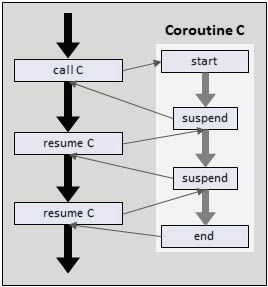
\includegraphics[width=0.6\textwidth]{content/chapter14/images/1.png}\\
Figure 14.1. Coroutines
\end{center}

different thread to where it was previously suspended. Coroutines are an orthogonal feature which, however, could be used together with multiple threads.

Effectively, using a coroutine is like having a function in the background that you start and continue from time to time. However, because the lifetime of a coroutine goes beyond nested scopes, a coroutine is also an object that stores its state in some memory and provides an API for dealing with it.

There are a few basic aspects in C++ regarding coroutines:

\begin{itemize}
\item 
Coroutines are defined implicitly just by using one of the following keywords in a function:

\begin{itemize}
\item 
co\_await

\item 
co\_yield

\item 
co\_return
\end{itemize}

In case none of these keywords is necessary inside a coroutine, you have to explicitly write a co\_return; statement at the end.

\item 
A coroutine usually returns an object that serves as the coroutine interface for the caller. Depending on the purpose and use of the coroutine, that object can represent a running task that suspends or switches context from time to time, a generator that yields values from time to time, or a factory that returns one or more values lazily and on demand.

\item 
Coroutines are stackless. You cannot suspend an inner coroutine that was called within an outer coroutine without suspending the outer coroutine. You can only suspend the outer coroutine as a whole.

When a coroutine is suspended, the state of the coroutine as a whole is stored in an object separately from the stack so that it can be resumed in a totally different context (in a different call stack, in another thread, etc.).
\end{itemize}












